\newpage
\subsection{Multi-compartment Imaging} \label{sec:multi}

In this final module you will integrate everything you have learned in this lab to probe a multi-compartment phantom using spectroscopy, projections, and 2D imaging.

\textbf{Use the agar + oil phantom throughout this module.}

%\textbf{Use the water + oil phantom until directed otherwise}. Please take care to keep this phantom upright so as to preserve the separation of water and oil.

\vspace{5mm}
\noindent \emph{Re-calibrate the center frequency before any lengthy imaging sequence for best image quality.}

% \begin{wrapfigure}{r}{0.5\textwidth}
%     \vspace{-5mm}
%     \centering
%     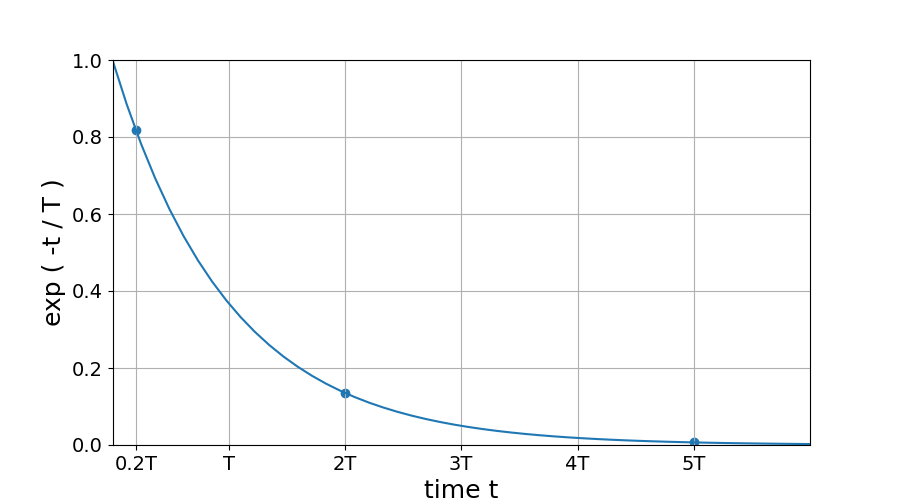
\includegraphics[width=0.5\textwidth]{exp-decay}
%     \captionsetup{width=0.4\textwidth}
%     \caption{\label{fig:decay} Exponential decay with a generic time constant $T$. This plot can serve as a reference for designing efficient relaxometry experiments.}
% \end{wrapfigure}



\subsubsection{Spectroscopy}

We begin by inspecting the spin echo spectrum for this multi-compartment phantom.

\begin{enumerate}
\item	In the main menu, click \textbf{Spectroscopy} and select the \textbf{Spin Echo} sequence.
\item	Open \textbf{Parameters}. Under \emph{General} set TE to 10 ms, Sampling Time to 6 ms.
\item	Click \textbf{Acquire}, then \textbf{Data Process}.
\end{enumerate}

\color{red}
\noindent You learned in class that the resonant frequency of fatty tissue (oil here) differs from watery tissue (agar here) due to an electron shielding effect called chemical shift. Why do we only see one peak in the spectrum? How \emph{could} this experiment be modified to resolve the two peaks (without changing the phantom itself)? Hint: your answer may well go beyond the current capabilities of the tabletop system by changing/improving hardware or software.
\color{black}
% soln: increase sampling time to improve spectral resolution, but also need better B0 homogeneity for this to actually help. Or, use a stronger main field to increase the spectral separation. Or introduce a gradient to spatially resolve the two, then rely on contrast (e.g. T1, T2) to separate.

\subsubsection{Projection with $T_2$ Contrast} \label{sec:proj-T2}

%Now let's play with the signal contrast of two materials having significantly different $T_2$: water and oil.
Now let's begin to play with $T_2$ contrast:

\begin{enumerate}
    \item   In the main menu, click \textbf{Projections} and select the \textbf{Spin Echo (On Axis)} sequence.
    \item   Open \textbf{Parameters}. Under \emph{General}, set TE to 10 ms, Sampling Time to 6 ms. Under \emph{Imaging}, set Image Resolution to 64 and FOV to 30 mm. Under \emph{Projections}, select only Y (the bore axis).
    \item   Click \textbf{Acquire}, then \textbf{Data Process}.
    \item   Observe the resulting projection plot. Adjust the frequency range to better visualize the signal profile. You should find that the two materials are nearly indistinguishable with these timing parameters.
    \item   Now try repeating the scan for several larger values of TE to increase the contrast. Do not change any other parameters. Observe how the relative signal levels change between the two materials.
\end{enumerate}

\color{red} \noindent
Include screenshots of the projection plot for three values of TE showing a range of contrast from low to high.
\color{black}
\vspace{5mm}

\color{red}
\noindent
Explain why these values of TE lead to different contrasts. Derive an expression for the optimal TE maximizing $T_2$ contrast between any two materials. Use the $T_2$ values you measured in the relaxometry module to compute the optimal TE for this case. How does this optimal TE compare with what you found empirically?
\color{black}
% soln: TE = log(T2_oil / T2_agar) / (1/T2_agar - 1/T2_oil)

\subsubsection{2D Imaging with $T_2$ Contrast} \label{sec:2d-T2}

Now that you have achieved $T_2$ contrast, let's see how it looks in a 2D image.

\begin{enumerate}
    \item   In the main menu, click \textbf{Imaging} and select the \textbf{2D Spin Echo} sequence.
    \item   Open \textbf{Parameters}. Under \emph{General}, set TR to 5000 ms, Sampling Time to 6 ms. Set TE for maximal T2 contrast between the two materials (use what you found in section \ref{sec:proj-T2}). Under \emph{Imaging}, set Image Orientation to XY, Image Resolution to 32 pixels, FOV to 30 mm.
    \item   Click \textbf{Acquire}. After it runs, click \textbf{Data Process}.
    \item   Observe the resulting images. \emph{If you are using ocra1 you will find the image y axis is flipped relative to the lab frame (bright agar appears on top).}
    \item   Repeat the above steps for a different TE value exhibiting minimal contrast.
    
    \color{red} Screenshot the resulting images for both TE values.
    \color{black}
 
    \item Repeat one of the above scans with Sampling Time 1 ms and 12 ms.

\color{red} \noindent
    Compare the set of images with different sampling times. Explain any differences. Hint: in order to cover the same k-space extent the readout gradient amplitude must be inversely proportional to the sampling time.
\color{black}
    
\end{enumerate}


\subsubsection{2D Imaging with $T_1$ Contrast} \label{sec:2d-T1}

% Try repeating section \ref{sec:proj-T2} with an agar + oil phantom (no write-up necessary). You will find it is much harder to distinguish agar \& oil because the $T_2$ value are more similar. Hence we will explore $T_1$ weighting as an alternative means of contrast for this phantom.

Now we will explore $T_1$ weighting as an alternative means of contrast for this phantom.

\begin{enumerate}
    \item   In the main menu, click \textbf{Imaging} and select the \textbf{2D Spin Echo} sequence.
    \item   Open \textbf{Parameters}. Under \emph{General}, set TE to 10 ms, Sampling Time to 6 ms. Under \emph{Imaging}, set Image Orientation to XY, Image Resolution to 32 pixels, FOV to 30 mm.
    \item   Design TR values to achieve (i) no contrast and (ii) high contrast between the two materials. Use the $T_1$ values you measured in the relaxometry module to inform your design. \emph{Note: the Relax 2.0 software limits TR to a minimum of 500 ms.}
 \end{enumerate}

 \color{red} \noindent
 Include screenshots of the resulting images with no/high $T_1$ contrast.
 \color{black}

\subsubsection{2D Imaging with $T_1$ Nulling} \label{sec:2d-T1}

Fat signal can be a nuisance for clinical MRI, so many techniques have been developed to remove this signal. One such approach is called TI-nulling. This approach uses an inversion recovery (IR) sequence with the inversion time (TI) parameter tuned to suppress a particular $T_1$ species. We will use this approach to suppress the ``fat'' signal in this phantom.

\color{red}
Calculate the TI needed to null the oil signal using the $T_1$ you measured in the relaxometry module. Hint: you should have already derived the necessary equation for this calculation in the relaxometry module. Your sketch of the sequence may also be helpful to reference.
\color{black}
% soln: TI=T1*log(2)
% around 70 ms

\begin{enumerate}
    \item   Navigate to the main menu. Click \textbf{Imaging} and select the \textbf{2D Inversion Recovery (SE)} sequence.
    \item   Open \textbf{Parameters}. Under \emph{General}, set TE to 10 ms, set TI to the fat-nulling value you found, Sampling Time to 6 ms, TR to 5000 ms. Under \emph{Imaging}, set Image Orientation to XY, Image Resolution to 32 pixels, FOV to 30 mm.
    \item   Click \textbf{Acquire}. After it runs, click \textbf{Data Process}.
 \end{enumerate}

\noindent{}\color{red}
Include a screenshot of the fat-suppressed images.
\color{black}


